\documentclass[13pt, a4paper, twoside]{article}
\usepackage[utf8]{inputenc}
\usepackage{geometry}
\usepackage[czech]{babel}
\usepackage{chemformula}
\usepackage{chemfig}
\usepackage{enumitem}
\usepackage{float}
\usepackage{fancyhdr}
\usepackage{caption}
\usepackage{setspace}
\usepackage{multicol}
\geometry{legalpaper, margin=1.05in}
\pagestyle{fancy}
\lhead{\Large Šárka Doležalová, skupina 6}
\rhead{\large 10.12.2020}
\begin{document}
\begin{center}
    \Huge
    Úloha 10: Stanovení rozpustnosti a obsahu krystalové vody
\end{center}
\large \onehalfspacing
\section*{Zadané úlohy}
\begin{enumerate}
    \item Stanovte rozpustnost předloženého vzorku anorganické soli ve vodě při laboratorní teplotě.
    \item Na základě naměřených údajů identifikujte neznámý vzorek.
    \item Termogravimetricky stanovte množství krystalové vody v předloženém vzorku.
\end{enumerate}

\section*{Teoretický úvod}
\subsection*{Rozpustnost látek}
Gibbsův zákon fází popisuje rovnováhu v uzavřeném systému rovnicí: $f+v = s +2 $.
ve které je f počet fází, v počet stupňů volnosti a s počet složek v systému. Fáze jsou homogenní složky (plyn, kapalina, pevná fáze) systému a složky jsou jednotlivé chemické sloučeniny. Stupeň volnosti je jakákoliv intenzivní fyzikální veličina. Intenzivní veličina je taková, která nezávisí na celkové hmotě systému.

\subsection*{Krystalová voda}
Když látky krystalizují z vodném prostředí do sebe často zabudovávají molekuly vody do struktury krystalu. Krystalové vody se může snadno zbavit stáním krystalických vzorků na vzduchu.

\subsection*{Práce s automatickou pipetou}
Automatická pipeta se používá o odměření velmi malých objemů. Daný objem se nastavuje šroubem v horní části pipety. Pipetu nesmíme nikdy obracet napo pokládat na stranu, pokud je na ní nasazena znečištěná špička.

\subsection*{Zahřívání nad kahanem a žíhání do konstantní hmotnosti}
Žíhání je specifickým laboratorním postupem provádějícím se nad kahanem, obvykle v porcelánových miskách. Kelímek je zahříván pomalu, aby nepraskl, poté je přesunut do nejteplejší části plamene. K žíhání můžeme také používat žíhací pec.
Žíhání do konstantní hmotnosti můžeme využít například při gravimetrii. 

\section*{Postup}
\subsection*{Stanovení rozpustnosti a identifikace vzorku}
Nad kahanem byly vyžíhány tři kelímky do konstantní hmotnosti. Žíhání probíhalo cca 10 minut a kelímky byly pomocí kleští přesunuty do exsikátoru k vychladnutí. Vychladlé kelímky byly zváženy na analytických vahách. Žíhání kelímků bylo zopakováno. Kelímky byly znovu zváženy a hmotnosti byly porovnány. Kdyby se hmotnosti měnili, proces by byl zopakován. Byla změřena teplota suspenze neznámého vzorku (č.105), poté co byl vzorek rozmíchán a bylo počkáno 5 minut. Do vyžíhaných kelímků bylo pomocí automatické pipety odpipetováno 5 ml nasyceného roztoku a byla zapsána hmotnost roztoku. Voda z odpipetovaných roztoků byla opatrně odpařena. Po odpaření vody, byl zbytek v kelímcích žíhán ještě dalších 10 minut. Po vychladnutí v exsikátoru byly kelímky zváženy a kelímky byly žíhány do konstantní hmotnosti.

\subsection*{Plamenová zkouška}
Předem vyžíhaný drátek byl ponořen do neznámého vzorku a poté byl vložen do plamene. Podle jeho barvy byl určen kationt v roztoku.

\subsection*{Stanovení obsahu krystalové vody}
V peci vyhřáté na 400°C byly vyžíhány dva malé kelímky do konstantní hmotnosti. Bylo postupováno stejně jako v předchozí úloze. Na analytických vahách do nich bylo odváženo přibližně 250 mg (viz naměřené hodnoty) neznámého vzorku. Odvážené vzorky, byly žíhány v peci při teplotě 400°C po dobu 10 minut.

\section*{Naměřené hodnoty}
\begin{figure}[H]
    \centering
    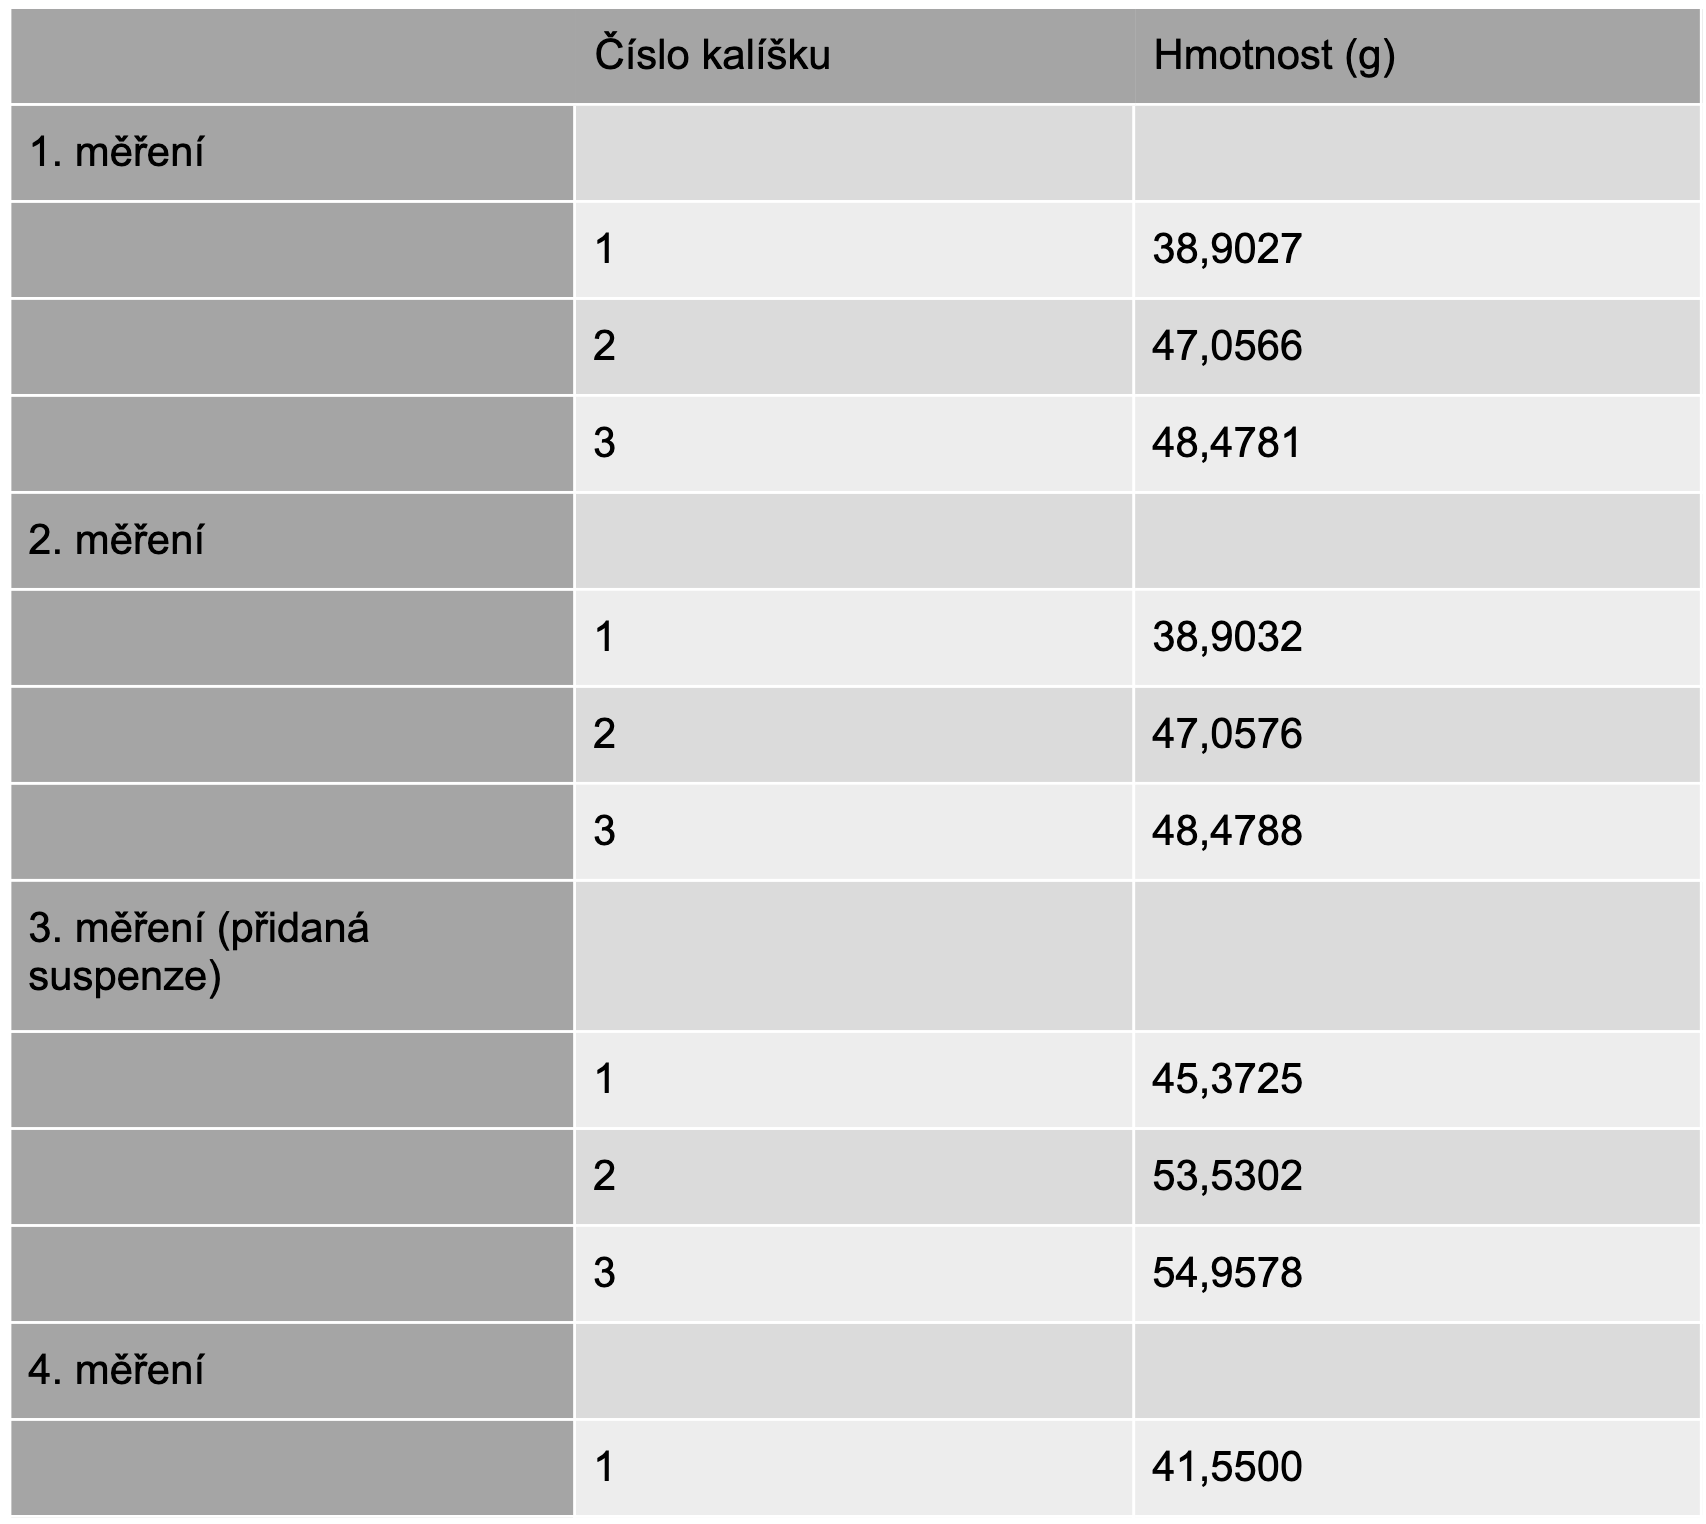
\includegraphics[width=6.8in]{tab_uloha10_1.png}
\end{figure}

\begin{figure}[H]
    \centering
    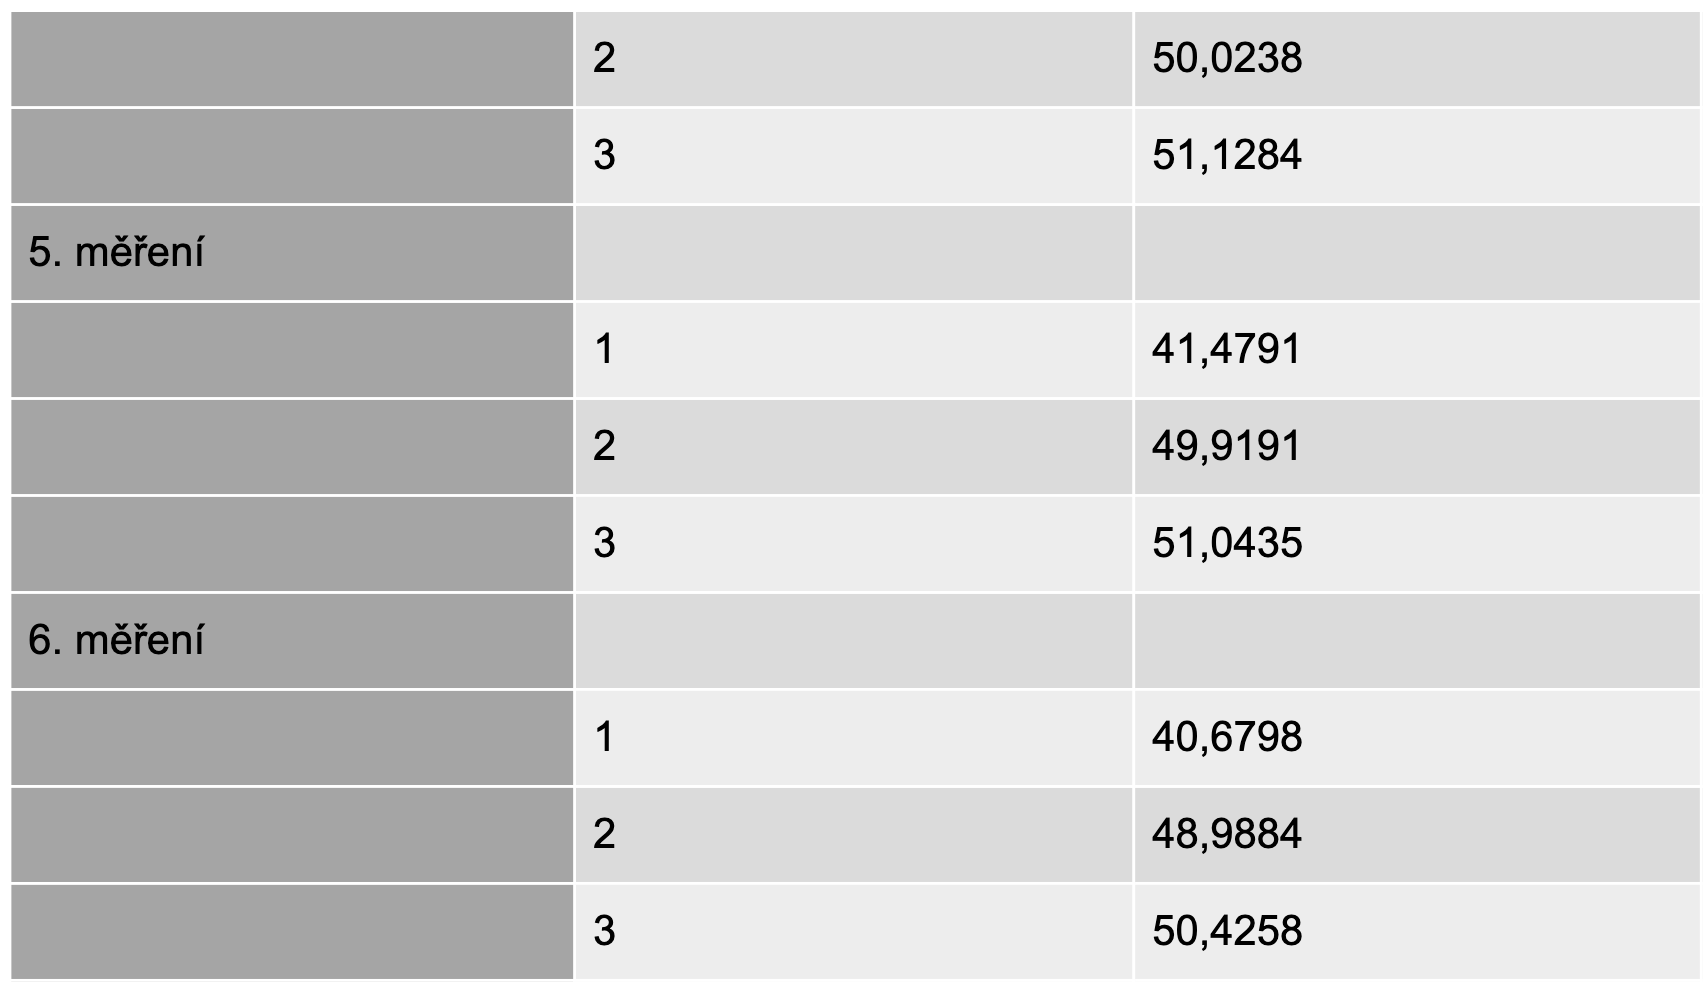
\includegraphics[width=6.8in]{tab_uloha10_2.png}
    \caption*{Tab. 1: žíhání do konstantní hmotnosti při stanovení rozpustnosti a identifikace roztoku
    }
\end{figure}

\begin{figure}[H]
    \centering
    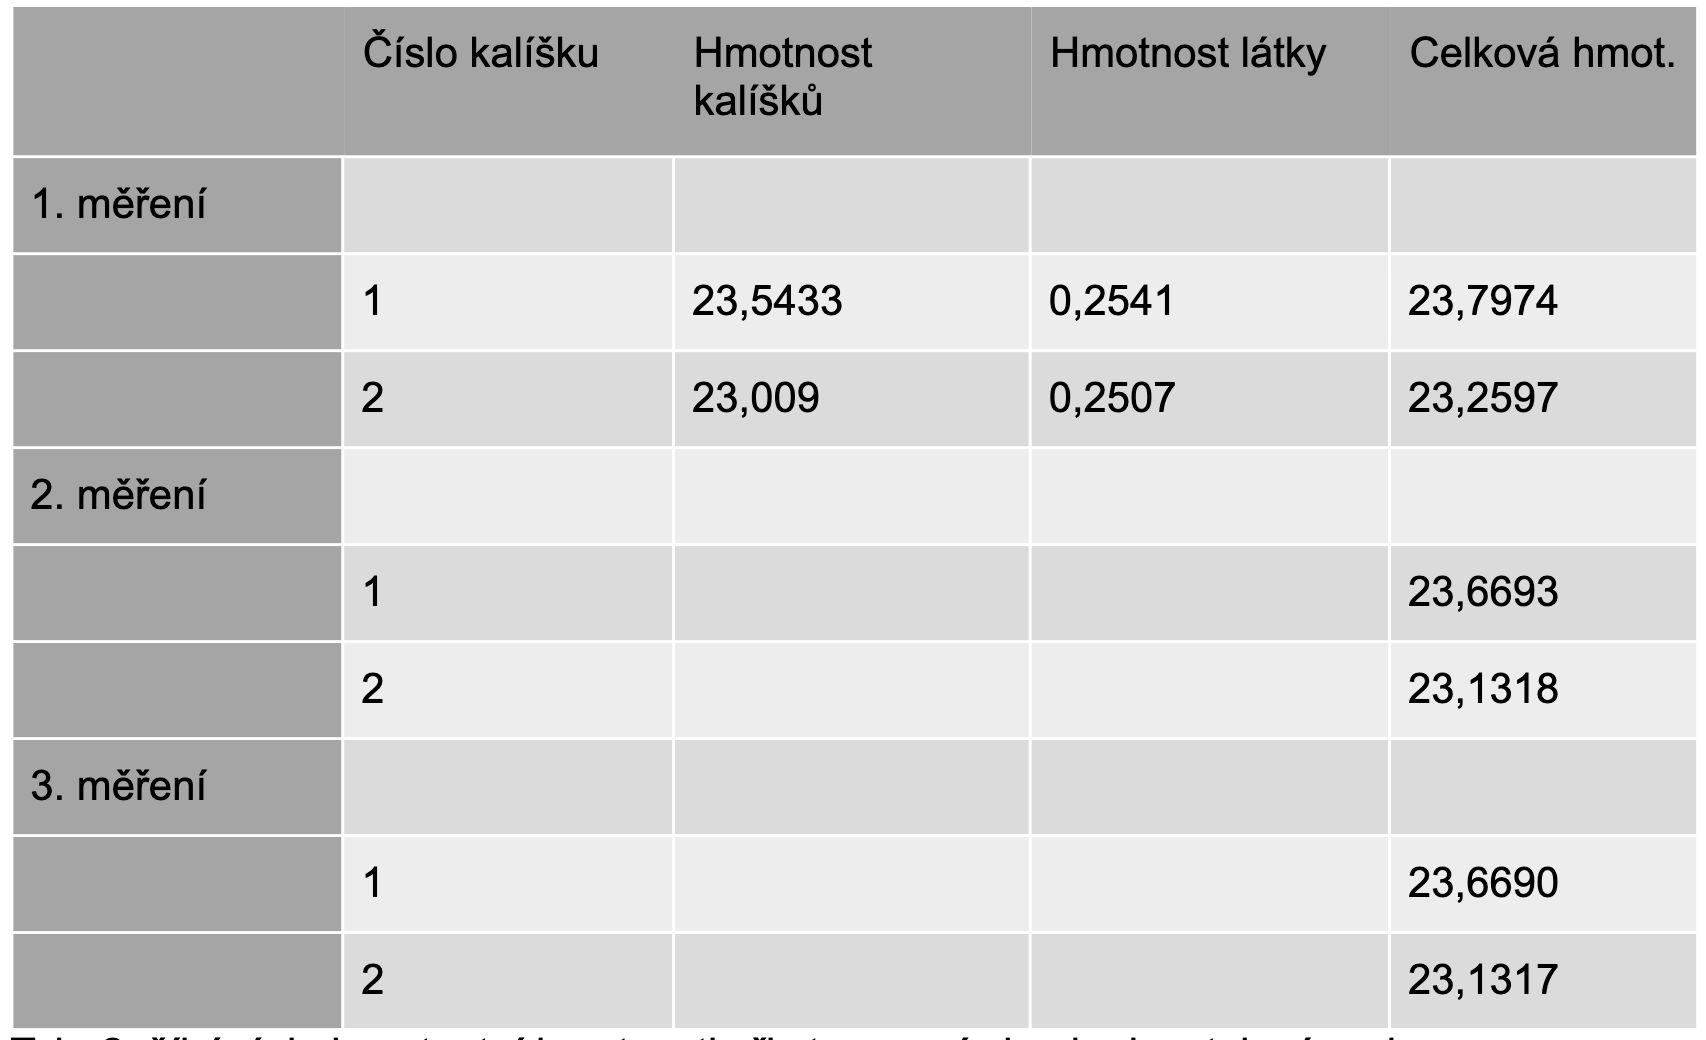
\includegraphics[width=6.8in]{tab_uloha10_3.png}
    \caption*{Tab. 2: žíhání do konstantní hmotnosti při stanovení obsahu krystalové vody}
\end{figure}

\section*{Výpočty}
\subsection*{Stanovení rozpustnosti a identifikace vzorku}
\begin{align*}
    m_{1(vzorek)}&=6,4693\: g\\
    m_{2(vzorek)}&= 6,479\: g\\
    m_{3(vzorek)}&= 6,479\: g
\end{align*}

\begin{align*}
    m_{1(výtěžek)}
\end{align*}







\end{document}